\documentclass[red]{beamer}
\usetheme{Warsaw}

% Fonts and encoding: pdfLaTeX needs inputenc/fontenc, LuaLaTeX and XeLaTeX use fontspec.
\usepackage{iftex}
\ifPDFTeX
    \usepackage[T1]{fontenc}
    \usepackage[utf8]{inputenc}
    \usepackage{lmodern}
\else
    \usepackage{fontspec}
\fi
\usepackage[polish]{babel}

\usepackage{amsmath}
\usepackage{graphicx}
\usepackage{booktabs}
\usepackage{listings}
\usepackage{tikz}
\graphicspath{{../figs/}}

% No section navigation bar at the top and no navigation symbols.
\setbeamertemplate{headline}{}
\setbeamertemplate{navigation symbols}{}

% Footline: a thin progress bar above the usual Warsaw split line (authors | title),
% with the slide number added on the right.
\setbeamertemplate{footline}{%
    \leavevmode%
    \begin{tikzpicture}
        \fill[red!15] (0, 0) rectangle (\paperwidth, 1.5pt);
        \fill[red!65!black] (0, 0) rectangle ({\insertframenumber / \inserttotalframenumber * \paperwidth}, 1.5pt);
    \end{tikzpicture}%
    \par\nointerlineskip%
    \hbox{%
        \begin{beamercolorbox}[wd=.5\paperwidth,ht=2.5ex,dp=1.125ex,leftskip=.3cm,rightskip=.3cm plus1fil]{author in head/foot}%
            \usebeamerfont{author in head/foot}\insertshortauthor%
        \end{beamercolorbox}%
        \begin{beamercolorbox}[wd=.5\paperwidth,ht=2.5ex,dp=1.125ex,leftskip=.3cm plus1fil,rightskip=.3cm]{title in head/foot}%
            \usebeamerfont{title in head/foot}\insertshorttitle\hspace{1.5em}\insertframenumber/\inserttotalframenumber%
        \end{beamercolorbox}}%
}

\lstset{
    language=Python,
    basicstyle=\ttfamily\scriptsize,
    keywordstyle=\bfseries\color{red!60!black},
    commentstyle=\itshape\color{gray},
    stringstyle=\color{green!40!black},
    columns=fullflexible,
    keepspaces=true,
    showstringspaces=false,
    frame=single,
    rulecolor=\color{gray!50},
    xleftmargin=2pt,
    xrightmargin=2pt,
    aboveskip=2pt,
    belowskip=4pt,
}

\title[GHRS: reprodukcja, FCM i SVD++]{GHRS: Graph-based Hybrid Recommendation System with Application to Movie Recommendation}
\subtitle{Miękkie metody klastrowania w~grafowo-hybrydowych systemach rekomendacyjnych}
\author[K. Kostka, R. Jarzyński, M. Jeżewski, M. Gagoś]{
    Kamil Kostka \and
    Radosław Jarzyński \and
    Maciej Jeżewski \and
    Michał Gagoś
}
\date{Lublin, \today}

\begin{document}

    \begin{frame}
    \titlepage
    \end{frame}

    \section{Wstęp}
    \begin{frame}{Motywacja i~cel}
        \small
        \begin{itemize}
            \item System rekomendacyjny przewiduje ocenę $\hat r_{ui}$, jaką użytkownik $u$
                  wystawiłby filmowi $i$
            \item Nowy użytkownik nie ma historii ocen - problem \textbf{zimnego startu}
            \item Systemy hybrydowe uzupełniają oceny informacją poboczną: demografią,
                  strukturą grafu, gatunkami filmów
            \item Miara jakości na zbiorze testowym $T$:
                  \[
                      \mathrm{RMSE} = \sqrt{\frac{1}{|T|} \sum_{(u, i) \in T} \left(r_{ui} - \hat r_{ui}\right)^2}
                  \]
        \end{itemize}
        \begin{block}{Pytanie badawcze}
            Czy grafowa reprezentacja użytkowników połączona z~klastrowaniem przewiduje
            oceny trafniej niż klasyczne modele?
        \end{block}
    \end{frame}

    \begin{frame}{Artykuł bazowy: architektura GHRS}
        \centering
        % Top half of the paper's diagram: steps 1-5, the user representation.
        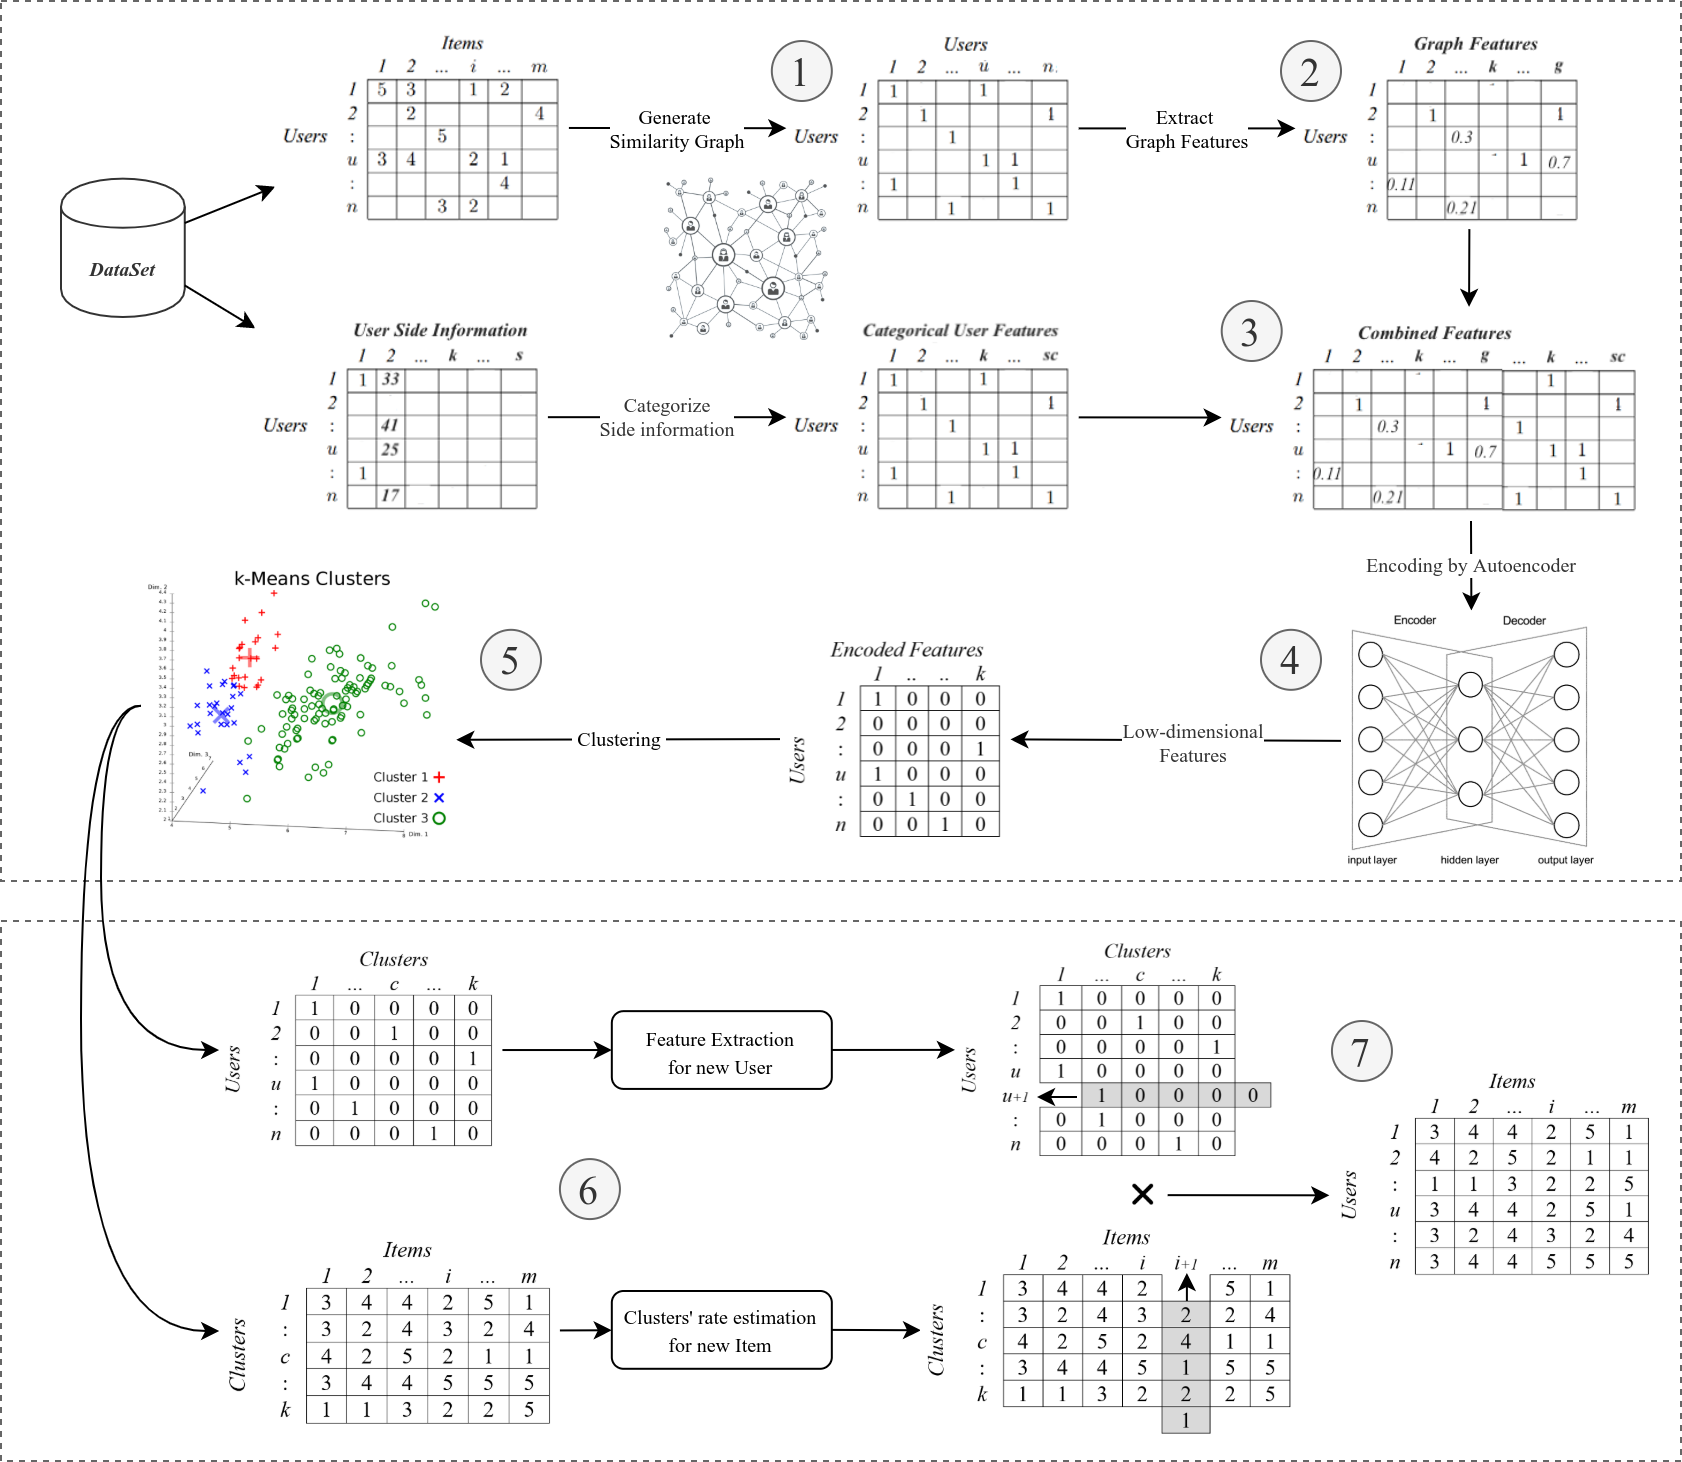
\includegraphics[width=\textwidth, trim=0 574 0 0, clip]{ghrs-structure.png}\\[1pt]
        {\scriptsize\itshape Źródło: Darban i~Valipour, Expert Systems with Applications (2022)}\\[5pt]
        \footnotesize
        \begin{tabular}{@{}ll@{}}
            (1)~Graf podobieństwa & (4)~Autoenkoder 35-16-4-16-35 \\
            (2)~Sześć miar centralności & (5)~K-Means w~przestrzeni kodów ($K = 8$) \\
            (3)~Demografia: razem 35 cech & (6-7)~Przypisanie średniej oceny klastra \\
        \end{tabular}
    \end{frame}

    \begin{frame}[fragile]{Zbiór danych: MovieLens 100K}
        \begin{center}
            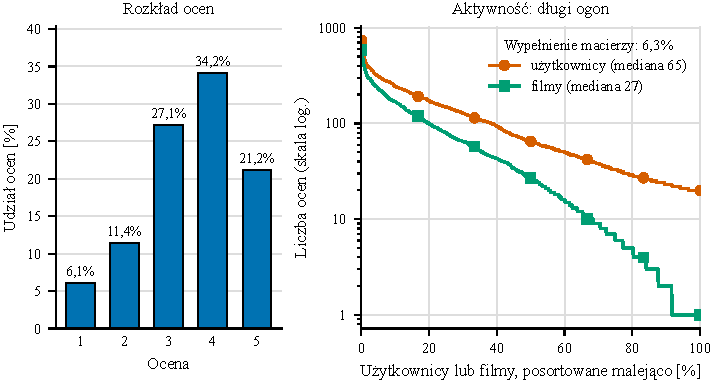
\includegraphics[width=0.84\textwidth]{fig0_dataset_exploration.pdf}
        \end{center}
        \vspace{-4pt}
        \begin{columns}[T]
            \begin{column}{0.5\textwidth}
                \scriptsize
                \begin{itemize}
                    \item 943 użytkowników, 1682 filmy, 100\,000 ocen w~skali 1-5
                    \item Macierz ocen pusta w~93,7\%; każdy użytkownik ma co najmniej
                          20 ocen, a~141 filmów tylko jedną
                    \item Metadane: wiek, płeć i~zawód użytkownika, 19 gatunków filmu
                \end{itemize}
            \end{column}
            \begin{column}{0.46\textwidth}
\begin{lstlisting}[language={},basicstyle=\ttfamily\tiny]
>>> ratings = load_ratings("u.data")
>>> ratings.shape
(100000, 4)
>>> ratings.head(3)
   UID  MID  rate       time
0  196  242     3  881250949
1  186  302     3  891717742
2   22  377     1  878887116
\end{lstlisting}
            \end{column}
        \end{columns}
    \end{frame}

    \section{Audyt i~reprodukcja}
    \begin{frame}{Deklarowany wynik a~reprodukcja}{MovieLens 100K, 5-krotna walidacja krzyżowa (u1-u5)}
        \small
        \begin{center}
            \begin{tabular}{lccc}
                \toprule
                \textbf{GHRS} & \textbf{RMSE} & \textbf{Precyzja} & \textbf{Czułość} \\
                \midrule
                Wynik z~artykułu & $0{,}887$ & $0{,}771$ & $0{,}799$ \\
                Nasza reprodukcja & $1{,}076 \pm 0{,}001$ & $0{,}664$ & $0{,}724$ \\
                \bottomrule
            \end{tabular}
        \end{center}
        \begin{itemize}
            \item Autorzy udostępnili tylko kod kroków 1-3; autoenkoder, K-Means
                  i~klastrową regułę wyznaczania ocen odtworzyliśmy według opisu
            \item Graf i~cechy budowane osobno dla każdego foldu, wyłącznie na danych
                  treningowych; 5 ziaren losowych
            \item Strojenie parametrów nieopisanych w~artykule (Optuna) oraz
                  17 wariantów autoenkodera: RMSE $1{,}025$-$1{,}079$
            \item Deklarowane $0{,}887$ byłoby lepsze od faktoryzacji macierzy
                  ($0{,}935$ na tych samych foldach)
        \end{itemize}
    \end{frame}

    \begin{frame}{Audyt: skąd może pochodzić wynik $0{,}887$?}{Symulacja naszych hipotez błędów ewaluacji}
        \begin{center}
            \footnotesize
            \begin{tabular}{lc}
                \toprule
                \textbf{Hipoteza ($K = 8$)} & \textbf{RMSE} \\
                \midrule
                H0: poprawny protokół & $1{,}075$ \\
                H1: graf z~danych treningowych i~testowych & $1{,}067$ \\
                H4: ewaluacja na danych treningowych & $0{,}935$ \\
                H3: oceny testowe w~średnich klastrów & $0{,}942$ \\
                H3 przy $K \approx 20$-$24$ & $0{,}877$-$0{,}890$ \\
                \midrule
                Najlepszy podział wybrany z~użyciem etykiet testowych & $0{,}902$ \\
                \bottomrule
            \end{tabular}
        \end{center}
        \small
        \begin{itemize}
            \item $0{,}887$ pojawia się wyłącznie przy wycieku ocen testowych
                  i~przy $K \approx 22$ zamiast $K = 8$
            \item Nawet wtedy precyzja i~czułość nie zgadzają się z~artykułem
        \end{itemize}
        \begin{block}{Wniosek}
            Punktem odniesienia dla dalszych prac jest RMSE $1{,}076$ (baseline: AE + K-Means)
        \end{block}
    \end{frame}

    \section{Wkład własny}
    \begin{frame}{Wkład własny: przegląd}
        \small
        \begin{enumerate}
            \item \textbf{GMM, FCM:} miękkie przypisanie użytkownika do $K$~klastrów
            \item \textbf{VAE:} wariacyjny autoenkoder w~miejsce klasycznego
            \item \textbf{Graf z~warunkiem TF-IDF:} podobne oceny i~profil gatunkowy
            \item \textbf{SVD++ z~cechami GHRS:} klastry korygują błędy tego modelu
        \end{enumerate}
        \begin{block}{Rygor eksperymentalny}
            \footnotesize
            \begin{itemize}
                \item \textbf{Rozdzielenie modułów:} reprezentację (AE, VAE), graf
                      i~klastrowanie wymieniamy pojedynczo przy niezmienionej regule
                      predykcji; ten sam moduł klastrowy działa potem na błędach SVD++
                \item \textbf{Warianty kontrolne:} partycje FCM i~GMM jako twarde etykiety
                      (argmax), graf z~tą samą liczbą losowych krawędzi, model bez klastrów
                      ($K = 1$), same obciążenia użytkownika i~filmu
                \item \textbf{Protokół:} te same foldy i~ziarna, hiperparametry ustalone
                      przed testem, sparowany test $t$ z~poprawką Nadeau i~Bengio oraz
                      korektą Holma
            \end{itemize}
        \end{block}
    \end{frame}

    \begin{frame}[fragile]{Miękkie klastrowanie: GMM i~FCM}
        \footnotesize
        \begin{itemize}
            \item FCM: waga klastra maleje z~odległością, $u_{uc} \propto d_{uc}^{-2/(m-1)}$;
                  współczynnik rozmycia $m > 1$ steruje miękkością
            \item GMM: waga to prawdopodobieństwo a~posteriori $p(c \mid z_u)$
            \item Prognoza to średnia ocen klastrów ważona przynależnością:
                  $\hat r_{ui} = \sum_{c} u_{uc}\, CI_{ci}$
        \end{itemize}
        Implementacja (\texttt{ghrs/clustering\_soft.py}, \texttt{ghrs/recommender.py}):
\begin{lstlisting}
def _fcm_weights(d2: np.ndarray, m: float) -> np.ndarray:
    logw = -np.log(np.maximum(d2, 1e-12)) / (m - 1.0)
    w = np.exp(logw - logw.max(axis=1, keepdims=True))
    return w / w.sum(axis=1, keepdims=True)

p = GaussianMixture(n_components=k, ...).fit(X).predict_proba(X)

w = self.UC[u]
SUM = np.stack([np.bincount(i, w[:, c] * e, self.n_items)
                for c in range(K)])
CNT = np.stack([np.bincount(i, w[:, c], self.n_items)
                for c in range(K)])
pred = base + np.einsum("nk,kn->n", self.UC[u], self.CI[:, i])
\end{lstlisting}
        Dla wag 0/1 model sprowadza się dokładnie do predykcji z~artykułu, opartej
        na średniej ocenie w~klastrze.
    \end{frame}

    \begin{frame}[fragile]{Reprezentacja generatywna: wariacyjny autoenkoder}
        \footnotesize
        \begin{itemize}
            \item Koder $35 \rightarrow 16 \rightarrow (\mu, \log\sigma^2) \in \mathbb{R}^4$,
                  dekoder $4 \rightarrow 16 \rightarrow 35$, optymalizator Nadam
            \item Funkcja straty: błąd rekonstrukcji i~dywergencja KL względem $\mathcal{N}(0, I)$
            \item Do klastrowania używamy średniej rozkładu a~posteriori $\mu$
        \end{itemize}
        Implementacja (\texttt{ghrs/autoencoder\_vae.py}):
\begin{lstlisting}
class KLDivergence(layers.Layer):
    def call(self, inputs):
        z_mean, z_log_var = inputs
        kl = -0.5 * ops.sum(1.0 + z_log_var - ops.square(z_mean)
                            - ops.exp(z_log_var), axis=-1)
        self.add_loss(self.beta * ops.mean(kl))
        return z_mean

class Sampling(layers.Layer):
    def call(self, inputs, training=None):
        z_mean, z_log_var = inputs
        eps = keras.random.normal(ops.shape(z_mean),
                                  seed=self.seed_generator)
        return z_mean + ops.exp(0.5 * z_log_var) * eps
\end{lstlisting}
    \end{frame}

    \begin{frame}[fragile]{Graf użytkowników z~warunkiem TF-IDF}
        \footnotesize
        \begin{itemize}
            \item Profil gatunkowy $t_u$: liczba ocenionych filmów każdego z~19 gatunków,
                  ważona TF-IDF i~znormalizowana
            \item Krawędź $(u, v)$ wymaga obu warunków: te same oceny dla co najmniej
                  $\alpha \cdot 1682$ filmów oraz $\cos(t_u, t_v) \geq 0{,}95$
            \item Kontrola: graf z~tą samą liczbą losowo zachowanych krawędzi
        \end{itemize}
        Implementacja (\texttt{ghrs/graph\_tfidf.py}):
\begin{lstlisting}
uid, mid = df_ratings["UID"], df_ratings["MID"]
A = sp.csr_matrix((np.ones(len(uid)), (uid, mid)),
                  shape=(n_users + 1, n_items))
counts = np.asarray(A @ G)
tfidf = TfidfTransformer().fit(counts[has_ratings])
profiles = tfidf.transform(counts).toarray()

cos = profiles @ profiles.T
rows, cols = similar_pairs(S, C, alpha_coef, mode, n_items)
keep = cos[rows, cols] >= cos_threshold
\end{lstlisting}
    \end{frame}

    \begin{frame}[fragile]{SVD++ z~cechami GHRS i~korekta klastrowa}
        \footnotesize
        \begin{itemize}
            \item Przypisanie użytkownikowi średniej oceny jego klastra pomija obciążenia:
                  czy użytkownik ocenia surowo, czy film jest lubiany;
                  same obciążenia $\mu + b_u + b_i$ dają RMSE $0{,}946$
            \item SVD++ łączy obciążenia, czynniki ukryte i~listę ocenionych filmów
                  z~35 cechami GHRS oraz 19 gatunkami
            \item Klastry uczą się błędów SVD++ wyznaczonych modelami, które nie widziały
                  danej oceny; przy małej liczbie ocen korekta znika ($\lambda = 25$)
        \end{itemize}
        Uproszczony fragment (\texttt{ghrs/experiment.py}, \texttt{ghrs/factorization.py}):
\begin{lstlisting}
svdpp = SVDppConfig(k=32, lam=0.1, seeds=(42, 0, 1))
for s in svdpp.seeds:
    svd = fit_svdpp(train, U, G, svdpp, s)
    eval_pred.append(svd.predict(test))
    train_pred.append(out_of_fold_predictions(train, U, G, svdpp, s))
train_offset = np.mean(train_pred, axis=0)
eval_offset = np.mean(eval_pred, axis=0)

rec = RecConfig(baseline="offset", similar="none",
                fallback="baseline", shrink=25.0)
model = ClusterRatingModel(rec).fit(train, UC, genres,
                                    offset=train_offset)
pred, tiers = model.predict(test, offset=eval_offset)
\end{lstlisting}
    \end{frame}

    \section{Wyniki}
    \begin{frame}{Wyniki: porównanie RMSE}{MovieLens 100K, 5-krotna walidacja krzyżowa (u1-u5)}
        \begin{center}
            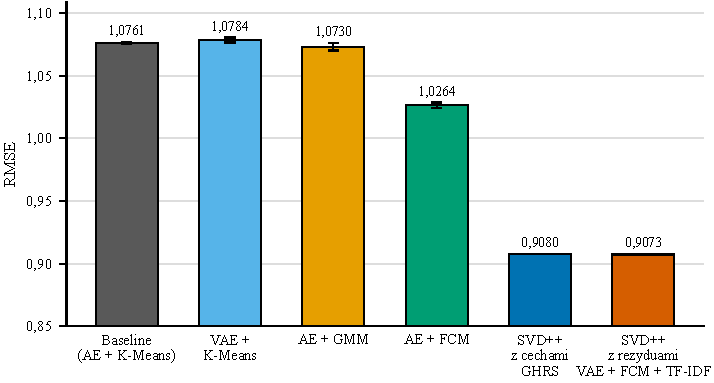
\includegraphics[width=0.78\textwidth]{fig1_rmse_comparison.pdf}
        \end{center}
        \footnotesize
        \begin{itemize}
            \item \textbf{AE + FCM:} $1{,}076 \rightarrow 1{,}026$ we wszystkich 5 foldach
                  ($p < 0{,}001$); AE + GMM ($1{,}073$) i~VAE + K-Means ($1{,}078$) bez poprawy
            \item \textbf{SVD++ z~cechami GHRS:} $0{,}908$, o~$0{,}168$ lepiej niż baseline
                  (5/5 foldów, $p < 10^{-6}$)
            \item \textbf{Korekta klastrowa:} FCM poprawia SVD++ we wszystkich 5 foldach
                  ($-0{,}0006$, $p = 0{,}04$), pełny zestaw osiąga $0{,}907$; twarde
                  K-Means nie poprawia
        \end{itemize}
    \end{frame}

    \begin{frame}{Mechanizm poprawy FCM: wygładzanie w~stronę średniej}{MovieLens 100K, model AE + FCM}
        \begin{center}
            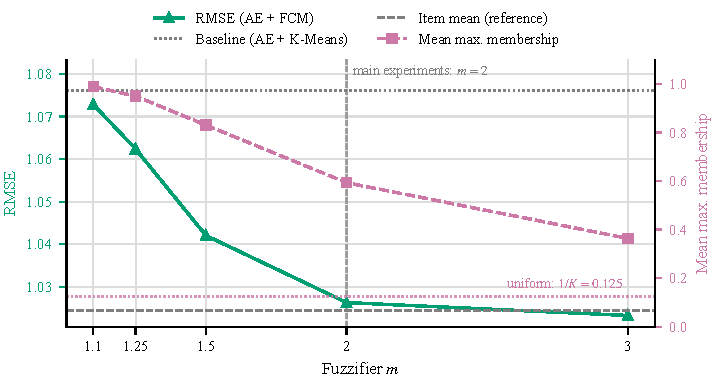
\includegraphics[width=0.74\textwidth]{fig2_fuzziness.pdf}
        \end{center}
        \footnotesize
        \begin{itemize}
            \item Większe $m$ spłaszcza wagi ($m = 3$: maks.\ waga $0{,}36$ przy
                  $1/K = 0{,}125$), a~prognoza $\sum_c u_{uc} CI_{ci}$ zbliża się
                  do średniej ocen filmu ze wszystkich klastrów
            \item Te same partycje FCM użyte jako twarde etykiety dają $1{,}077$: zysk
                  wynika z~wygładzania prognozy, a~nie z~lepszego podziału użytkowników
        \end{itemize}
    \end{frame}

    \begin{frame}{Weryfikacja: podział temporalny i~test wycieku}{MovieLens 100K}
        \begin{center}
            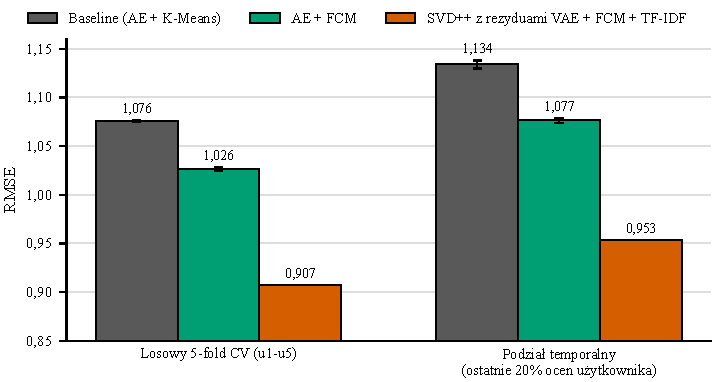
\includegraphics[width=0.74\textwidth]{fig4_temporal_robustness.pdf}
        \end{center}
        \footnotesize
        \begin{itemize}
            \item Podział temporalny przewiduje ostatnie 20\% ocen każdego użytkownika
                  z~wcześniejszych, jak w~działającym systemie: błędy rosną, kolejność
                  modeli się nie zmienia, korekta FCM nadal pomaga ($-0{,}0012$)
            \item Permutacja ocen testowych zmienia prognozy o~$7 \cdot 10^{-6}$, poniżej
                  szumu numerycznego; przy celowym wycieku (H3) o~$4{,}1$
        \end{itemize}
    \end{frame}

    \section{Wnioski}
    \begin{frame}{Wnioski}
        \small
        \begin{enumerate}
            \item \textbf{Ograniczeniem GHRS jest klastrowa reguła predykcji, a~nie
                  reprezentacja:}
                  te same 35 cech GHRS w~modelu SVD++ daje RMSE $0{,}908$ zamiast $1{,}076$
            \item \textbf{Miękkie klastrowanie działa jak regularyzacja:} samodzielnie
                  obniża RMSE o~$0{,}05$, a~jako korekta SVD++ daje stabilną poprawę
                  we wszystkich foldach i~w~podziale temporalnym
            \item \textbf{Miękkie przypisanie wygrywa z~twardym:} FCM poprawia SVD++,
                  K-Means nie
            \item \textbf{VAE i~graf TF-IDF} nie wnoszą mierzalnego zysku ponad FCM
            \item \textbf{Zimny start pozostaje otwarty:} dla nowych użytkowników
                  najlepsze modele osiągają RMSE około $1{,}03$
        \end{enumerate}
    \end{frame}

    \begin{frame}{Podsumowanie i~kod źródłowy}
        \small
        \begin{center}
            \footnotesize
            \begin{tabular}{lc}
                \toprule
                \textbf{Model} & \textbf{RMSE} \\
                \midrule
                GHRS (wynik deklarowany) & $0{,}887$ \\
                Baseline: reprodukcja GHRS (AE + K-Means) & $1{,}076$ \\
                AE + GMM & $1{,}073$ \\
                VAE + GMM & $1{,}064$ \\
                AE + FCM & $1{,}026$ \\
                VAE + FCM + TF-IDF & $1{,}025$ \\
                SVD++ z~cechami GHRS & $0{,}908$ \\
                SVD++ z~korektą VAE + FCM + TF-IDF & $0{,}907$ \\
                \bottomrule
            \end{tabular}\\[2pt]
            {\scriptsize Średnie z~5 foldów (u1-u5) i~3 ziaren losowych}
        \end{center}
        \begin{itemize}
            \item \textbf{Dalsze prace:} dobór $K$, $m$ i~$\lambda$ na zbiorze walidacyjnym,
                  zbiór MovieLens 1M, modele cech dla zimnego startu
        \end{itemize}
        \begin{block}{Kod źródłowy}
            \url{https://github.com/KaloeSan/ghrs-soft-clustering}\\[2pt]
            {\scriptsize Python 3.14, PyTorch, scikit-learn; wszystkie wyniki i~wykresy
            generowane skryptami}
        \end{block}
    \end{frame}

\end{document}
